\documentclass[11pt, oneside]{article}   	% use "amsart" instead of "article" for AMSLaTeX format
\usepackage{geometry}                		% See geometry.pdf to learn the layout options. There are lots.
\geometry{letterpaper}                   		% ... or a4paper or a5paper or ... 
%\geometry{landscape}                		% Activate for rotated page geometry
%\usepackage[parfill]{parskip}    		% Activate to begin paragraphs with an empty line rather than an indent
\usepackage{graphicx}				% Use pdf, png, jpg, or eps§ with pdflatex; use eps in DVI mode
								% TeX will automatically convert eps --> pdf in pdflatex		
\usepackage{amssymb}
\usepackage{color}
\newcommand{\todo}[1]{ \textcolor{red}{\bf{To Do:} #1}}
\newcommand{\toref}[1]{ \textcolor{blue}{\bf{REFERENCE #1}}}
%SetFonts

%SetFonts


\title{6 Month TAP Report}
\author{By Me :)}
\date{}							% Activate to display a given date or no date

\begin{document}
\maketitle

\section{Wounds and Plasma Treatment}
Plasmas are rapidly extending into the field of medicine, with potential applications for wound healing \cite{Haertel2014nonthermal, Isbary2013nonthermal}, cancer treatment \cite{Hirst2016low, Fridman2007floating}, coagulation \cite{Fridman2006blood, Chen2009blood} and sterilisation \cite{Fridman2006blood, Laroussi2002nonthermal}.
Applications such as there pertain to plasmas ability to interact with living biological substrates such as bacteria, both in planktonic and biofilm forms \cite{Joshi2010control, Pei2012inactivation, Ziuzina2015cold} and eukaryotic, mammalian cells \cite{Haertel2014nonthermal}.
For sterilisation applications, the properties of low temperature plasma, in particular the low temperature and ability to operate at atmospheric pressure, allow their use both on equipment surfaces \cite{Laroussi2002nonthermal} and also directly on biological tissue, for example chronically infected wounds \cite{Haertel2014nonthermal, Isbary2013nonthermal, Fridman2006blood}.

This project is concerned with wound healing and how low temperature air plasma can be developed to allow treatment of wounds.
Plasmas can be used on wounds with two aims:
\begin{enumerate}
\item Bacterial killing
\item Host cell activation and healing promotion
\end{enumerate}

While exact mechanisms of action are not fully understood, there have been investigations into the roles of the different plasma components.
Briefly, low temperature plasmas are very weakly ionised gases (degree of ionisation $<$ 1\%), with a global temperature of of approximately room temperature ($< 40^{\circ} C$), and dry reactive environment, allowing direct contact with biological substrates.
Electrons liberated in the plasma mediate the different plasma components, for example, dissociation of molecules, yielding reactive radical species, emission as a result of electron impact electronic excitation and ionisation which yields ions and allows plasma sustainment.
It is, therefore, likely that the efficacy seen so far using plasmas is due to this complex plasma composition, and also what suggests that bacteria are going to be less likely to build up resistance, due to the multimodal nature of the plasma treatment.

The main three components that will be discussed in the next sections are charged particles and associated electric fields, emission of, for example UV photons, and reactive neutral species.


\subsection{Bacterial Killing}
\subsubsection{RONS}
LTP is a highly efficient source of reactive species, produced by mechanisms such as electron impact excitation and dissociation.
The gas present in the plasma determines the types of species that will be produced. 
In the case of air plasma, reactive oxygen and nitrogen species (RONS) are readily produced and these have multiple possible effects on biological substrates.
Important species produced include atomic oxygen (O), ozone (O$_3$), singlet delta oxygen (O$_2$($^1\Delta$)), superoxide (O$_2^-\cdot$), atomic nitrogen (N), hydroxyl radicals (OH), hydrogen peroxide (H$_2$O$_2$) and various nitrogen oxides (NO, NO$_2$ and N$_2$O) \cite{Graves2014low}.

Whilst reactive species were thought to be purely damaging molecules produced in the body which only serve to promote disease and ageing \cite{Harman1955aging}, it is now known that their role is far more complex than this, and that reactive species have crucial roles to play in the immune system and in normal physiological signalling \cite{Thannickal2000reactive}.
At low concentrations, RONS are vital to human health. 
For example, they are important cell signalling regulating molecules in cells such as fibroblasts, endothelial cells and smooth muscle cells.
Further to this, they are essential for host defence as they are produced by immune cells during an immune response in order to kill invading pathogens.
The importance of this function is shown by patients with chronic granulomatous disease (CGD), who cannot synthesise the superoxide radical (O$_2^-\cdot$) resulting in multiple, persistent infections \cite{PhamHuy2008free, Fang2004antimicrobial}.


If the concentrations of RONS become excessive and there is an imbalance between radical formation and neutralisation, then they can become dangerous, causing damage to lipids, proteins and DNA \cite{PhamHuy2008free}.
Considering plasma treatments containing ROS, these exogenous species can enter the cells, or induce the formation of new ROS intracellularly and exert their action \cite{Haertel2014nonthermal}.
RONS can be visualised inside cells using fluorescent dyes, an example of which is shown by the likes of Joshi \textit{et al} \cite{Joshi2010control}.

Oxidative attack on lipids inside cells or as part of cell membranes results in a chain reaction and the formation of harmful products, the most mutagenic and toxic being malondialdehyde (MDA) and 4-hydroxynonenal (4-HNE), respectively \cite{Ayala2014lipid}.
Lipid peroxidation occurs as a chain reaction, mediated by free radicals, with the hydroxyl radical ($\cdot$OH) being particularly effective.
Firstly, the radical breaks an unsaturated carbon bond in the lipid, abstracts a hydrogen and forms a lipid radical, which then readily reacts with oxygen to form a lipid peroxy radical.
The lipid peroxy radical can then attack another lipid and abstract a hydrogen, forming a new lipid radical and a lipid hydroperoxide. 
Thus the process propagates until antioxidants such as vitamin E can neutralise the radical species \cite{Ayala2014lipid}.

Proteins can be changed structurally and enzymes break \cite{PhamHuy2008free}.

As with lipid peroxidation, the $\cdot$OH radical is effective for damaging DNA. 
There are many ways it can interact with the components of DNA, in particular through reactions with the purines and pyrimidines of DNA.
Although the body has many DNA repair mechanisms in place, mutations as a result of the oxidative insult still occur.
These are often result in mispairing of DNA bases and subsequent transversion mutations.
For example, a common lesion formed in DNA is 8-OH-Gua (a guanine base that has been modified through attack by $\cdot$OH), which wrongly pairs with adenine and thus results in a G $\rightarrow$ T transversion mutation \cite{Dizdaroglu2012oxidatively}.
It readily reacts with nucleotide bases, which allows for frequent mutations 
DNA attack can cause mutations. \cite{PhamHuy2008free}.







\subsubsection{UV}
UV emission is known to be harmful at certain wavelengths and powers, and, as such, it has been used extensively for sterilisation purposes due to it's ability to interfere with DNA \cite{Laroussi2004evaluation}.
To investigate the effects of UV radiation emitted from plasmas, windows can be put between the plasma and the sample that allow specific wavelengths of UV radiation through, while blocking all other plasma components. 
Using these methods, there is evidence to suggest that the effects of UV radiation are negligable \cite{Laroussi2004evaluation, Dobrynin2009physical}.
There is currently a lack of safety guidelines relating to the safe dose of UV that can be applied to skin.
Whilst there are suggestions for undamaged skin, there is nothing for broken, damaged skin, therefore, keeping the UV emission as low as possible is probably advisable \cite{Isbary2013cold}.

\subsubsection{Charged Particles and Electric Fields}
As charged particles are generally confined within the strong electric fields within the plasma, they don't tend to travel far outside the plasma bulk.
This means that one method for delineating the roles of electric fields and particles from the other plasma components is by comparing direct (where the biological substrate is in direct contact with the plasma) and indirect (where the biological substrate is only exposed to the plasma effluent) plasma treatments.
Investigations such as this have suggested that charged particles or electric fields, or a combination of both, are important for bacterial killing as direct treatment is much more efficient that indirect treatment \cite{Fridman2007comparison}.
A proposed mechanism for this increased efficacy when charged particles are in contact with the biological sample came from Mendis $et al$ in 2000 \cite{Mendis2000a} who suggested that accumulation of ions on the membranes of cells could cause an electrostatic force greater than the tensile strength of the membrane causing rupture.
This was noted following the observations of Laroussi \textit{et al} \cite{Laroussi1999images} that showed morphological changes and lysis of the treated bacteria.
\todo{Look into electroporation mechanism. Is this just electroporation by plasmas???}

\subsection{Host Cell Activation and Healing Promotion}
It seems that the molecular interactions of plasmas are less well understood when considering the beneficial effects it has on host cells and tissues.
However, by considering the normal, physiological effects of plasma components that are produced endogenously, and the observed outcomes from wound treatment with LTP, mechanisms of action can be proposed.

It is generally accepted that low doses plasma treatment is good for stimulating effects - in the context of wound healing this would include things like increased proliferation and migration and DNA repair. 
This contrasts with higher doses which generally induce damaging/lethal effects such as cell death and DNA damage \cite{Haertel2014nonthermal}. 

There is evidence to show that plasma treatment could accelerate wound healing, both from laboratory experiments, and clinical trials.
For example, following scratch tests, 3T3 keratinocytes treated with plasma recovered and re-grew to confluence more quickly than untreated controls \cite{Tipa2011plasma}.
This suggests that plasma treatment can increase keratinocyte proliferation, something which has also been shown by changes in gene expression in HaCaT keratinocytes following plasma treatment \cite{Barton2013nonthermal}.
Clinically, devices such as KinPen and MicroPlaSter have shown promise when used on human patients, aiding healing without any obvious side-effects \cite{Isbary2013cold, Isbary2012successful, Isbary2010a, Bekeschus2016the}.


%Plasma seems to be toxic to lymphocytes but not neutrophils or monocytes due to strong oxidation in the cell membrane and cytosol. This may be beneficial as excessive lymphocytes are present in pathological wounds and, therefore, by removing them, it may promote healing \cite{Bekeschus2016the}.
%\toref{Kramer2013suitability, Haertel2014, Bender2012, Brehmer2015, Joshi, Kong2009}
Dealing with the groups of plasma components, there is proposed mechanisms of action for RONS and electric fields in wound healing.
However, the actions of RONS and electric fields discussed below is not determined using plasma treatment, therefore, it can only be proposed that the same actions are carried out by plasma-produced species rather than endogenously produced species.


\subsubsection{RONS}
There is much evidence showing the importance of RONS in the normal, physiological process of wound healing.
Throughout the different stages of healing, RONS have a role to play.
Firstly, RONS are important for coagulation through involvement in the release of tissue factor (TF), which triggers the clotting cascade. RONS are also important for platelet recruitment and activation, subsequent further release of ROS and more TF production \cite{Soneja2005role}.
It is possible that plasma derived RONS can also carry out this function, as shown by multiple studies of plasma on coagulation \cite{Fridman2006blood, Chen2009blood}.

RONS are also important for the inflammatory, re-epithelialisation and wound contraction stages of wound healing.
This is particularly due to their ability to act as signalling molecules and also their role in mediating the release of factors and receptor affinity.
These roles help control chemotaxis and adhesion of immune cells recruited to the wound site and help the activation and proliferation of keratinocytes to start re-epithelialisation of the wound \cite{Soneja2005role}.
RONS are also involved in collagen production and control of myofibroblast (the cells which contract to decrease the wound area) formation \cite{Soneja2005role}.


Nitric oxide (NO) is a very important species in wound healing and contributes to all the processes above.
The potential for using NO therapeutically for wound healing applications has been investigated.
For example Shekhter \textit{et al} \cite{Shekhter2005beneficial} used an air plasma device, named 'plason', to produce an NO-containing gas flow which was then used to treat wounds in rats. 
The NO was produced by a high temperature electric arc discharge, and then the gas was allowed to cool before being used on the wounds. 
Wounds treated with 'plason' showed accelerated healing compared to the control group.
However, what I find unclear is how they know there was only NO in the gas, surely other species would also be present in the gas?

%Inflammation: Following immune cell recruitment to the wound site, they produce many factors important for potentiating the immune response. Species such as H$_2$O$_2$ are important secondary messenger molecules for these factors and are, therefore, important during an immune response. RONS in general are also important for affecting chemotaxis and adhesion of immune cells such as neutrophils and monocytes \cite{Soneja2005role}.
%
%Re-epithelialisation: ROS are important for promoting collagenase expression (for wound remodelling) and epidermal growth factor (EGF) expression, which promotes the proliferation of keratinocytes into the wound site \cite{Soneja2005role}.
%
%Angiogenesis: ROS also play a role in promoting angiogenesis, matrix deposition and wound contracture, by enhancing the release of pro-angiogenic factors and enhancing its receptor affinity, stimulating the release of collagen and controlling the transition of fibroblasts to myofibroblasts (the cells which contract to make the wound site smaller) \cite{Soneja2005role}.


\subsubsection{Electric Fields}

Normal plasma membrances have a potential difference across them, due to the movement of ions across the membrane.
When epithelium is broken through wounding, the ion currents are disrupted and an electric field is established.
There is evidence to suggest that this electric field helps guide the migration of epithelial cells during healing \cite{Zhao2009electrical}.
Following this, there have been studies into the effects of using electric fields for the promotion of wound healing \cite{Thakral2013electrical, Messerli2011extracellular}.
However, as with plasma treatment, there is little understanding of the relation between 'dose' and outcomes etc, though looks promising.
Also all the different trials use different regimes and therefore comparison is difficult.
Lab trials show the importance of electrical currents/fields for wound healing, and there are clinical trials involving electric fields for wound healing that show promise \cite{Messerli2011extracellular}.
\todo{E field strengths?? Applied voltages?? Comparison to plasmas}
%The threshold field strength noticeable by cells is 4500 times smaller than that required for electroporation of skeletal muscle \cite{Messerli2011extracellular}.

\section{Work to Date: Plasma Modelling \& Benchmarking}
Use of GlobalKin, as presented in the previous TAP, this is a 0-Dimensional, global plasma chemistry model which calculates time evolution of plasma species, given specific geometry and plasma parameters.
For the last TAP I was just using Sandra's chemistry set to learn how to use the model and try to simulate some of the experiments I carried out during my rotation project.
However, since then I have been working towards building my own air chemistry set.
This is not a trivial task and therefore, I am starting with building a set for nitrogen.

\subsection{Nitrogen Chemistry Set}
Ta to Vasco Guerra for set from \cite{Kutasi2016tuning}.
\subsubsection{Species}
Included species included in Vasco: N, N$_2$, the first 17 vibrational states of ground state N$_2$ (N$_2$ (X, v = 0 - 17)), excited states of N$_2$ (N$_2$ (A), N$_2$ (B), N$_2$ (B'), N$_2$ (C), and a species N$_2$ (AP1S) which is the combination of N$_2$ (a), N$_2$ (a') and N$_2$ (w) (GlobalKin only contains cross sections for this collective species, rather than each of the three individual ones, therefore, for the time being, they have to be treated as one), excited N atoms (N ($^2$P) and N($^2$D) and ions N$_2$+, N$_4$+ and N$_2$ (B)+.
\subsubsection{Electron Impact Reactions}
In-built cross sections in GlobalKin
\subsubsection{VT reactions}
These are important reactions as they are important destruction mechanisms for vibrationally excited nitrogen molecules


\section{Plasma Sources}
When considering the plasma source to build for wound treatment, it would be of use to develop the source in a way that it is possible to model it well.
For example, 


Here I talk about geometries that I could use, specifically review air plasmas.
\subsection{Geometry}
\subsubsection{Dielectric Barrier Discharge}
Dielectric barrier discharges are so called due to having a dielectric barrier on one of the electrodes to limit the current flow and prevent the glow-to-arc transition. 
They can operate at atmospheric pressure using air and don't necessarily require a gas flow \cite{Fridman2013plasmamedicine}
They have been used extensively for applications such as ozone production and polymer treatment and more recently, for biomedical applications \cite{Fridman2013plasmamedicine, Brehmer2015alleviation}.
A typical DBD setup is shown in figure \ref{fig:DBD} \todo{Add a figure showing a DBD setup}.
DBDs have shown to be effective for bacterial killing and other biomedical applications such as blood clotting, and there have been clinical trials into their effectiveness for wound healing \cite{Daeschlein2012in, Fridman2006blood, Brehmer2015alleviation}. 

DBDs have to be operated using alternating current.


\todo{Speak with Jerome about air plasma designs. Something Sandra built to try with his nanosecond supply??}


\begin{figure}
\centering
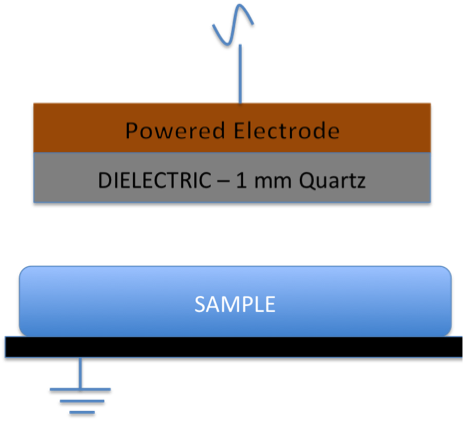
\includegraphics[width=0.5\textwidth]{Figures/DBD}
\caption{DBD}
\label{fig:DBD}
\end{figure}

DBDs have been shown in laboratory conditions to be effective for bacterial killing \cite{Daeschlein2012in, Fridman2006blood}.
An air DBD, PlasmaDerm has been tested on chronic ulcers in a clinical trial, though the results are not overly promising \cite{Brehmer2015alleviation}, as plasma induced killing of wound colonising bacteria was not long lasting and there did not appear to be any acceleration in wound healing in the plasma treated group compared to the controls.
The device operates at AC voltage pulses with amplitudes $>$10 kV and a power density of 120 mW/cm\textsuperscript{2} \cite{Brehmer2015alleviation}.



\cite{Fridman2007comparison} looks at direct and indirect plasma treatment. Using DBD with and without mesh/airflow to try and separate out the roles of ions and reactive species.
Both use atmospheric air as the gas.
Both operate at 35 kV, 12 kHz frequency and power density of 0.8 W/cm\textsuperscript{3}.

In terms of operation, there was a study investigating pulsing of DBD, using both micro- and nanosecond pulses. 
It was found that nanosecond pulsing gave a more homogenous plasma, that would ignite more uniformly over a non-uniform surface.
Specifically, patterned (i.e. not flat) agar was used as the target and it was seen that with microsecond pulses, the plasma was more filamentary and some areas didn't ignite at all \cite{Ayan2009application}. 
However, using the nanosecond pulses, the plasma was more uniform over the entire surface.
This is preferable when considering wound treatments, as the wound bed is not smooth.
Further to this, nanosecond pulsed DBD was found to be more effective for bacterial killing \cite{Ayan2008nanosecond}


\subsubsection{Floating-Electrode Dielectric Barrier Discharge}
Similar to DBD, the FE-DBD can be used whereby one of the electrodes can be replaced with anything with a sufficiently high charge storage capacity, a so-called, floating electrode (FE). 
Biological samples and skin are able to do this due to their high water content {\cite{Fridman2006blood}}.
Good diagrams of the electrodes are shown in {\cite{Fridman2006blood}}.
Has been shown that FE-DBD can accelerate the coagulation process in the blood. It seems to catalyse the physiological process of clotting rather than exerting a physical influence.
This is operated at 20 kV at pulsed and continuous frequency.

\subsubsection{Corona Discharge}
\cite{Dobrynin2011inactivation} - inactivation of bacteria using corona discharge.

\subsubsection{Plasma Jets}
\cite{Pei2012inactivation} - handheld air plasma 'Plasma Flashlight'
\cite{Chen2009blood} - Blood clotting trial using plasma jet
\cite{Walsh2011portable} - A portable air plasma ** Looks interesting!


\subsubsection{Voltages, Waveforms and Power etc}

Nanosecond pulsing.
Why? What is the point? What does it mean? Why is it necessary for air and less so for noble gas plasmas?



\section{Future Work}
\begin{itemize}
\item Add to chemistry set by adding in O$_2$. For now, I am only going to consider dry air, therefore only N$_2$:O$_2$ gas mixture.
\item EXPERIMENTS!!!!
\end{itemize}



\scriptsize
\bibliographystyle{ieeetr}
\bibliography{/Users/hld523/Bibliography/MyPapers}
\end{document}  